\section{\label{sec:calib}Calibration and Detector Performance}

The calibration of the raw data was done through seven incomplete but representative passes labeled \verb+pass0_v1+ through \verb+pass0_v7+ though only the last three of these is still available via JLab's mass storage system (\abbr{mss}). All calibration constants were put into the \mbox{\texttt{calib\_user.RunIndexg12}} run index with the exception of certain lepton-specific numbers as discussed in Sec.~\ref{sec:data.lepton}.

\subsection{\label{sec:calib.trig}Trigger}

\subsection{\label{sec:calib.trig.eff}Trigger Efficiency Study}

\begin{center} \color{OliveGreen}
This section is a verbatim excerpt from the dissertation by J.T.\ Goetz\cite{clas.thesis.goetz}.
\end{center}

In the first few weeks of \desg{g12}, during ``commissioning,'' an attempt to determine the efficiency of the two-track trigger (bit 8 in Tables.~\ref{tab:data.trig.conf.1} and \ref{tab:data.trig.conf.2}) was made. The rate of this main production trigger rose quadratically with the beam current while the physical event rate increased linearly. The number of accidentals, which must be cut from any analysis, increased with increasing current and at a certain point, the majority of the events taken were accidentals. The trigger rate as a function of the beam current is shown in Fig.~\ref{fig:data.trig.eff}. An estimate of the linear part of the trigger rate shows that approximately 60\% of the events recorded during the \desg{g12} experiment (which ran at 60--65~nA beam current) were accidentals.

\begin{figure}\begin{center}
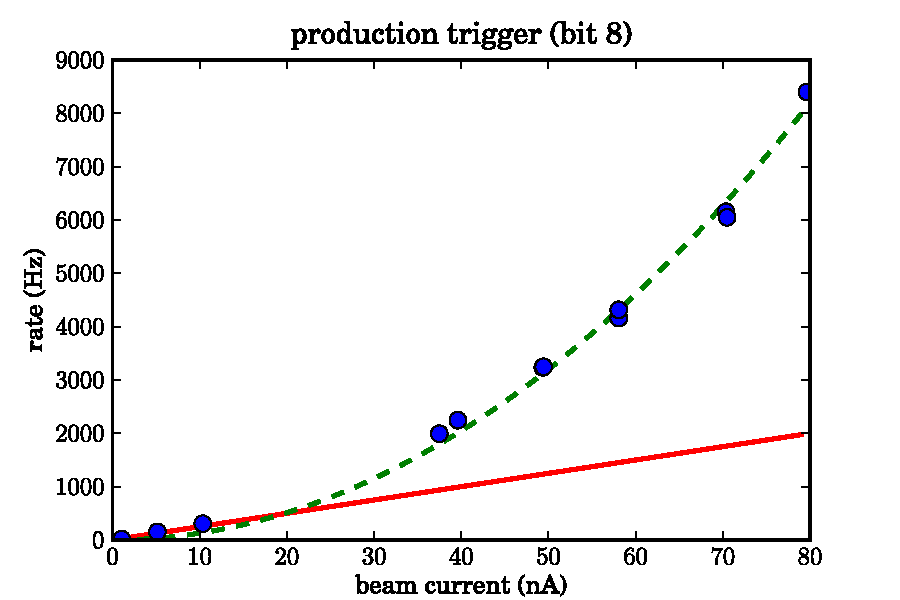
\includegraphics[width=0.7\columnwidth]{figures/calib/trig/trigger_study.eps}
\caption[Trigger Rate vs. Beam Current]{\label{fig:data.trig.eff}The production trigger rate (bit 8 in Tables~\ref{tab:data.trig.conf.1} and \ref{tab:data.trig.conf.2}) was measured for various beam currents shown by the blue dots. The rates below 10~nA are roughly linear and are extrapolated via the red solid line to show an estimate of the physical event rate. The actual trigger rate is fitted with a quadratic shown by the green dashed line. By this estimate, the accidental rate is shown to equal the physical event rate at approximately 40~nA. The \desg{g12} experiment was done at 60--65~nA.}
\end{center}\end{figure}

\FloatBarrier

\subsection{\label{sec:calib.tag}Tagger Timing Calibration}
The timing calibration of the tagger system was performed using the standard procedures. Overall, the quality of the calibration is excellent, showing an overall timing resolution of about $130~ps$, when the tagger time is compared with the RF time. The counter-by-counter alignment can be seen on Fig.~\ref{tagtpho}. The calibration was checked on a run by run basis (Fig.~\ref{tagRun}), and new constants were commissioned when major changes were noticed.  

\begin{figure}[h]
\begin{center}
 \includegraphics[width=0.45\textwidth]{figures/calib/tag/tagtpho.png}
  \caption{And example of the tagger timing calibration and the T-counter alignment, comparing  the difference between photon time determined from the tagger elements (T-counters, in this particular plot), and photon timing according to the RF. }
  \label{tagtpho}
  \end{center}
\end{figure}


\begin{figure}[h]
\begin{center}
 \includegraphics[width=0.45\textwidth]{figures/calib/tag/tagRun.png}
  \caption{The run-by-run behavior of the tagger timing calibration. Overall, the tagger timing resolution is about $130~ps$ for the production runs, and behaves stably throughout the running period.}
  \label{tagRun}
  \end{center}
\end{figure}

\subsection{Target Density}\label{sec:analysis.target_density}

We need to know the target density to calculate the differential cross-section. The procedure for determining the density of $\ell$H$_2$ target in \abbr{CLAS} has already been established in ~\cite{clas.target.density}. In the \desg{g12} experiment, the target temperature and pressure was measured periodically during each run. Each run contained at least 3 measurements of the pressure and temperature. The formula for calculating the target density is;
% ~\cite{clas.target.density}
\begin{align}
\rho = a_1T^2 + a_2P +a_3 \label{eq:target_density} \ ,
\end{align} 
where $T$ and $P$ represent the temperature and pressure respectively and $a_1$, $a_2$, $a_3$ are constants given in Tab.~\ref{tab:targetdensity} taken from ~\cite{mccarty}. Fig.~\ref{fig:target_density} shows the average target density, $\bar \rho$, for each run along with the $\sqrt{\sigma^2}$.
\begin{table}[h!]
\begin{minipage}{\textwidth}
\begin{center}
\begin{singlespacing}

\caption[Target Density Constants]{\label{tab:targetdensity}Constants used in target density measurements \vspace{0.75mm}}

\begin{tabular}{c|c}

%\hline \hline
%
%operation & \multicolumn{3}{c}{Generation} \\
%charge & I & II & III \\

\hline
Parameter & Value \\
\hline

$a_{1}$ & $-2.89 \cdot 10^{-5} \frac{g}{cm^3K^2}$  \\
$a_{2}$ & $1.0 \cdot 10^{-7} \frac{g}{cm^3mbar}$  \\
$a_{3}$ & $8.249 \cdot 10^{-2} \frac{g}{cm^3}$  \\
\hline \hline
\end{tabular}

\end{singlespacing}
\end{center}
\end{minipage}
\end{table}
\vspace{20pt}
The average density, for each run, was calculated as;
\begin{align}
\bar \rho_{run} = \frac{1}{N}\sum_i^N \rho_i \ ,
\end{align} 
while the variance $\sigma^2$ is calculated, for each run, as;
\begin{align}
\sigma^2 = \frac{1}{N - 1}\sum_i^N (\rho_i - \bar \rho)^2 \ .
\end{align}
Once the target density was calculated for each run, the average target density for all \desg{g12} runs was calculated using;
\begin{align}
\bar \rho_{tot} = \frac{1}{N_{run}}\sum_i^{N_{run}} \bar \rho_{run} = 0.0711398 \pm 1.74 \cdot10^{-5}\ ,
\end{align} 
while the variance $\sigma^2$ is calculated, for all \desg{g12} run, as;
\begin{align}
\sigma_{tot}^2 = \frac{1}{N_{run} -1}\sum_i^{N_{run}} (\bar \rho_{run} - \bar \rho_{tot})^2 = 0.00024 \ .
\end{align}
Since the uncertainty, $\sigma$, in the target density is lower than the uncertainty of the physical in the target materials, the target density uncertainty will not be a factor in the total systematic errors, Sec.\ref{sec:results.systematics}. The target length has an inaccuracy of 40~cm $\pm$ 0.2~cm. This gives a systematic of 0.5\%. 

\begin{figure}[h!]\begin{center}
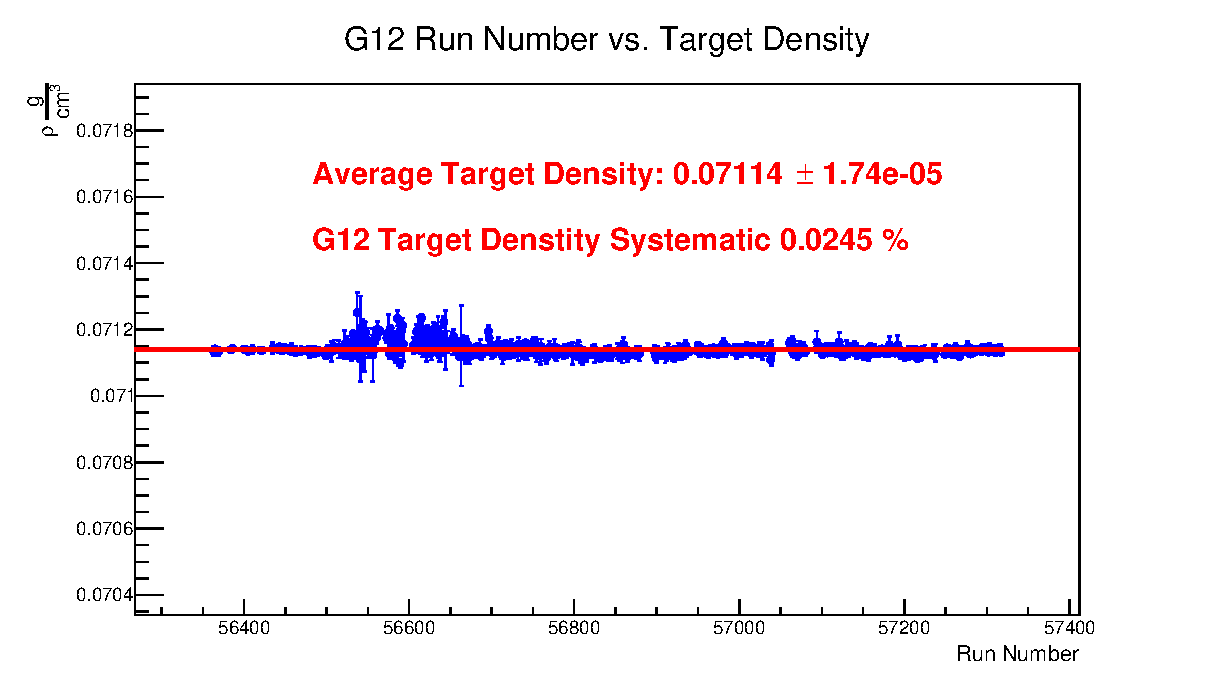
\includegraphics[width=0.9\textwidth]{figures/calib/targ/G12_Target_Density.eps}
\caption[Target density for \desg{g12}]{\label{fig:target_density}Target density for \desg{g12}. Image source:~\cite{clas.thesis.kunkel}}
\end{center}\end{figure}
\FloatBarrier
\subsection{\label{sec:calib.st}Start Counter Calibration and Resolution}

The start counter time-walk calibration took into account the varying geometry of the paddles. Fig.~\ref{fig:calib.st.adcuncor} shows the uncorrected timing difference for paddle 3 (of 24) as a function of \abbr{ADC} while Fig.~\ref{fig:calib.st.adccor} shows the corrected timing. This was done for each paddle and the resulting resolutions can be seen in Fig.~\ref{fig:calib.st.timepion} for pions, Fig.~\ref{fig:calib.st.timeproton} for protons, Fig.~\ref{fig:calib.st.timepion2d} for pions and all paddles, Fig.~\ref{fig:calib.st.timepion.ebeam} for pions a function of beam energy and Fig.~\ref{fig:calib.st.timepion.region} for pions as a function of geometry. The run-by-run resolution can be seen in Fig.~\ref{fig:calib.st.runbyrun}.

% ADC Uncorrected
\begin{figure}[htbp]\begin{center}
\includegraphics[width=0.65\columnwidth]{figures/calib/st/Uncorrected_adc.eps}
\caption[]{\label{fig:calib.st.adcuncor}}
\end{center}\end{figure}

% ADC Corrected
\begin{figure}[htbp]\begin{center}
\includegraphics[width=0.65\columnwidth]{figures/calib/st/Corrected_adc.eps}
\caption[]{\label{fig:calib.st.adccor}}
\end{center}\end{figure}

\begin{figure}[htbp]\begin{center}
\includegraphics[width=0.65\columnwidth]{figures/calib/st/Hpad3_sttag_pion.eps}
\caption[]{\label{fig:calib.st.timepion}}
\end{center}\end{figure}

\begin{figure}[htbp]\begin{center}
\includegraphics[width=0.65\columnwidth]{figures/calib/st/Hpad3_sttag_prot.eps}
\caption[]{\label{fig:calib.st.timeproton}}
\end{center}\end{figure}

\begin{figure}[htbp]\begin{center}
\includegraphics[width=0.6\columnwidth]{figures/calib/st/Hsttag_pion.eps}
\caption[]{\label{fig:calib.st.timepion2d}}
\end{center}\end{figure}

\begin{figure}[htbp]\begin{center}
\includegraphics[width=0.6\columnwidth]{figures/calib/st/Sterg_pion.eps}
\caption[]{\label{fig:calib.st.timepion.ebeam}}
\end{center}\end{figure}

\begin{figure}[htbp]\begin{center}
\includegraphics[width=0.6\columnwidth]{figures/calib/st/Timing_pad_3.eps}
\caption[]{\label{fig:calib.st.timepion.region}}
\end{center}\end{figure}

\begin{figure}[htbp]\begin{center}
\includegraphics[width=0.65\columnwidth]{figures/calib/st/STmeanandres_v5.eps}
\caption[]{\label{fig:calib.st.runbyrun}}
\end{center}\end{figure}

\FloatBarrier

As a check on the timing resolution of the start counter, we used data containing at least two K$^+$ (this was part of the cascade baryon search) to look at kaons, pion and protons at the same time. The momenta ($p$) of the tracks was given by the drift chamber and tracking algorithm found in the \bank{TBTR} bank, and the energy ($\Epid$) of the particle was set by particle identification. This allowed us to calculate the speed of the particle:
\begin{equation}
    \betapid = \frac{p}{\Epid}.
    \label{eqn:betapid}
\end{equation}
This was used to calculate the vertex time of the particle:
\begin{equation}
    \tvtofpid = \ttof - \frac{\ltof}{c\betapid},
    \label{eqn:tvtofpid}
\end{equation}
where $\ttof$ and $\ltof$ are the time and path length of the track at the \system{TOF} plane as obtained from the \bank{TDPL} bank. This time was converted to a ``photon time'' ($\tpho$) by subtracting the photon propagation time ($\tprop$) from the center of the target:
\begin{equation}
    \tphotofpid = \tvtofpid - \tprop,
    \label{eqn:tphotofpid}
\end{equation}
where
\begin{equation}
    \tprop = \frac{1}{c} \left( \ztgt - \zv \right),
\end{equation}
where $\ztgt$ is the center of the target's z-position ($-90$~cm in the \system{CLAS} coordinate system), and $\zv$ is the z-coordinate of the track's vertex position -- in this case, the intersection of the two kaons where the covariance matrixes of the estimated momenta are taken into account through the standard \prog{MVRT} vertexing algorithm. This photon time, $\tphotofpid$, was compared to the \system{RF}-corrected tagger times ($\ttgrf$) of each hit in the photon tagger as obtained from the \bank{TAGR} bank. The resulting data indicates a timing resolution of 310~ns for protons, 400~ns for pions, and 430~ns for kaons.

\begin{figure}[htbp]\begin{center}
\includegraphics[width=0.5\columnwidth]{figures/calib/st/dvertex_time_pid_st.pdf}
\caption[vertex timing, \abbr{TOF-ST} vs.\ \abbr{TOF-PID}]{\label{fig:dvertex_time_pid_st}Difference in vertex times for each track for the two calculations made above. Represents 1.5\% of the total statistics.}
\end{center}\end{figure}

\begin{figure}[htbp]\begin{center}
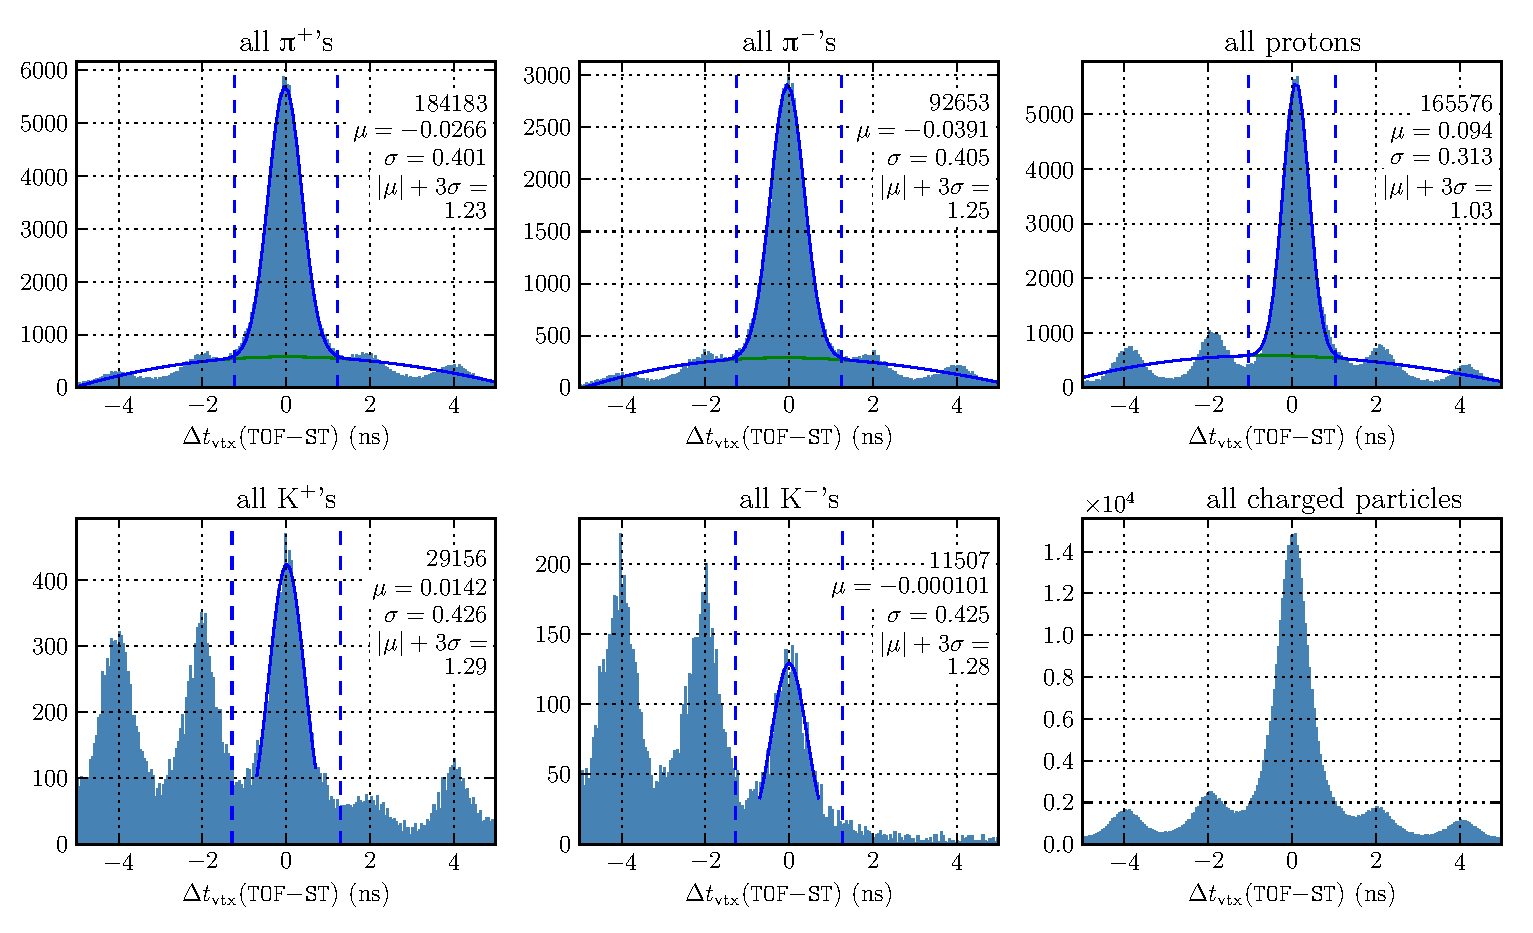
\includegraphics[width=0.9\columnwidth]{figures/calib/st/dvertex_time_st.eps}
\caption[vertex timing, \abbr{TOF-ST}]{\label{fig:dvertex_time_st}Difference in vertex time between that of the photon and of the tracks based on start counter and time-of-flight times. Represents 1.5\% of the total statistics.}
\end{center}\end{figure}


\subsubsection{\label{sec:calib.st.eff}Start Counter Efficiency}

The efficiency of the start counter was calculated by examining the number of tracks with a ST hit after track reconstruction. The ST fired $91.6\%$ of the time, this was calculated from run 57000 since it is a good run and included in production data.

\FloatBarrier

\subsection{\label{sec:calib.dc}Drift Chamber Calibration and Resolution}

\subsubsection{\label{sec:DC.TOF.res}Drift Chamber and TOF smearing parameters in \prog{gpp}}

Tracking in the Drift Chamber of a \abbr{CLAS} Sector is performed using the six superlayers of the \abbr{DC}. A good measure of the the quality of tracking are the \abbr{DC} residuals for each superlayer. After a track is identified using the hit elements in the \abbr{DC} superlayer, It's \abbr{DC} residual is calculated using the TBLA bank as follows:

\begin{verbatim}
fabs(TBLA->tbla[i].fitdoca) - fabs(TBLA->tbla[i].calcdoca)
\end{verbatim}

The values of the DC residuals in the CLAS data are empirically found to be a good fit to a convolution of 2 gaussians - a narrow gaussian and a broad gaussian. During DC calibrations efforts were made to minimize this residual to have maximum reconstruction efficiency. The mean and width of the residuals as a function of superlayer and run number are shown in Figs.~\ref{fig:calib.dc.residuals.mean} and \ref{fig:calib.dc.residuals.wid} respectively.


\begin{figure}\begin{center}
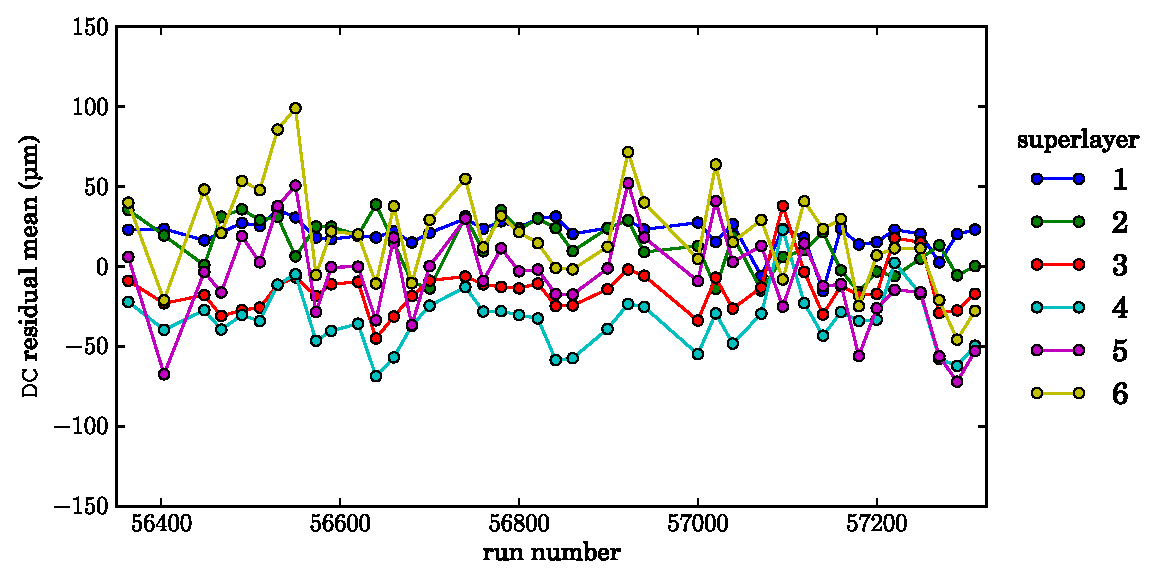
\includegraphics[width=0.6\textwidth]{figures/calib/dc/dc_resid_mean.eps}
\caption[DC Residuals (Mean)]{\label{fig:calib.dc.residuals.mean}Mean of residuals for the drift chambers by superlayer and by run.}
\end{center}\end{figure}

\begin{figure}\begin{center}
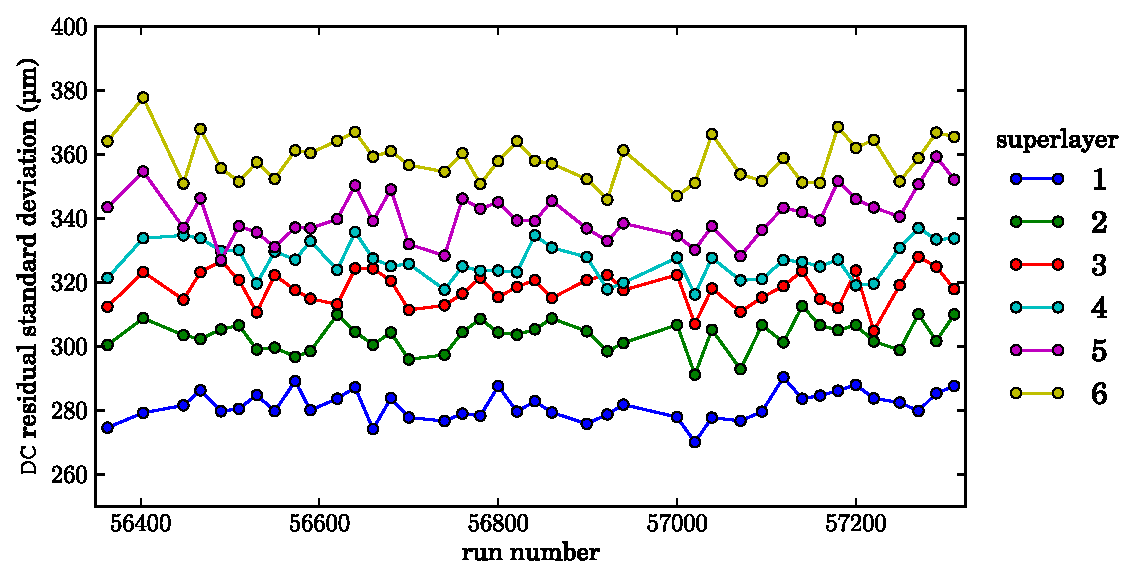
\includegraphics[width=0.6\textwidth]{figures/calib/dc/dc_resid_sigma.eps}
\caption[DC Residuals (Width)]{\label{fig:calib.dc.residuals.wid}Gaussian width of residuals for the drift chambers by superlayer and by run.}
\end{center}\end{figure}

\subsubsection{\label{sec:calib.dc.eff}Drift Chamber Wire Efficiency}
To generate the wiretap for g12, the utility pdu, available in SVN, was used. Maurizio Ungaro made the wiremaps for g12 with the root files [A01 and A02] for each run. These output files are at \url{/home/mukesh/work/pdu_hbook} at Jlab. Root files needed are at \url{/home/mukesh/work/pdu_root}. The values were added to the g12 database. The results of the wiretap are plotted in for each sector:

\begin{verbatim}
http://www.jlab.org/~ungaro/maureepage/proj/dceff/dc_periods/g12.html
\end{verbatim}

\FloatBarrier

%%%\subsection{\label{sec:calib.cc}Cerenkov Calibration and Resolution}

\subsubsection{\label{sec:calib.cc.eff}Cerenkov Efficiency}

\FloatBarrier

\subsection{\label{sec:calib.tof}Time-of-Flight Counter Calibration and Resolution}

\begin{itemize}
    \item The plots shown are for g12's run number 56855, pass0 v7. Did not change to pass1.
    \item Several steps were taken to calibrate the TOF for g12. Listed in C. Bookwalter's dissertation\cite{clas.thesis.bookwalter}:
    \begin{itemize}
        \item Counter status
        \item ADC pedestals
        \item TDC linearization constants
        \item Time-walk corrections
        \item Left-right delay constants
        \item Attenuation length
        \item Minimum-ionizing particle pulse heights
        \item Effective velocity
        \item Paddle-to-paddle offsets
    \end{itemize}
    \item The final time-walk corrections is a mix between constants from g6c and constants derived from g9a laser data using Gamecock.
    \item The plots (Figs.~\ref{plt:tofbetavpneg}--\ref{plt:tofrunbyrun}) included are:
    \begin{itemize}
        \item The TOF velocity ($\beta$) versus momentum by positive and negative tracks.
        \item The RF TOF by paddle ID by sector.
        \item The energy deposited versus momentum by positive and negative tracks.
        \item The TOF mass.
        \item The TOF resolution integrated over all paddles.
        \item The TOF run-by-run performance.
    \end{itemize}
\end{itemize}

\begin{figure}\begin{center}
    \begin{subfigure}{0.5\columnwidth}\begin{center}
        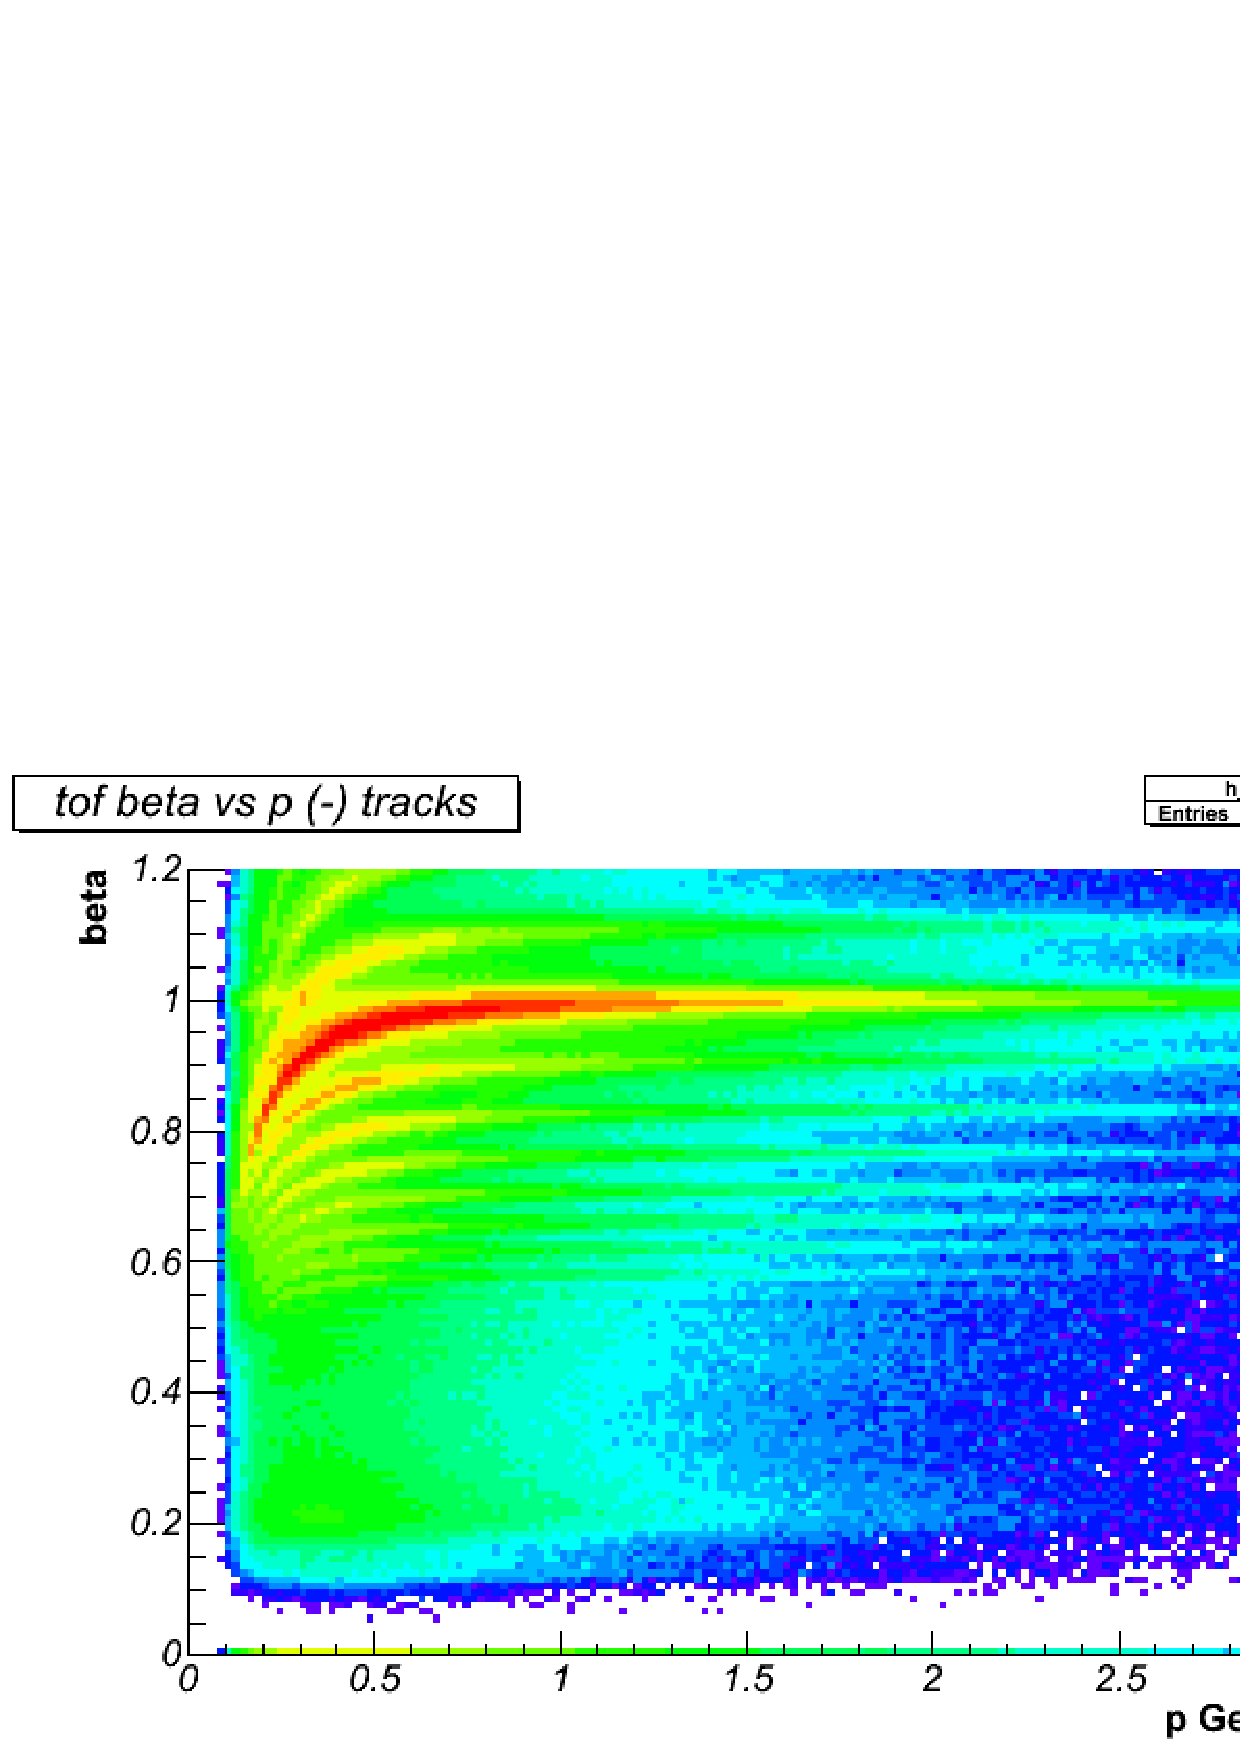
\includegraphics[width=.9\linewidth]{figures/calib/tof/Tof_56855_final_betavpm.pdf}
        \caption{TOF $\beta$ versus momentum for negative tracks}
        \label{plt:tofbetavpneg}
    \end{center}\end{subfigure}\begin{subfigure}{0.5\columnwidth}\begin{center}
        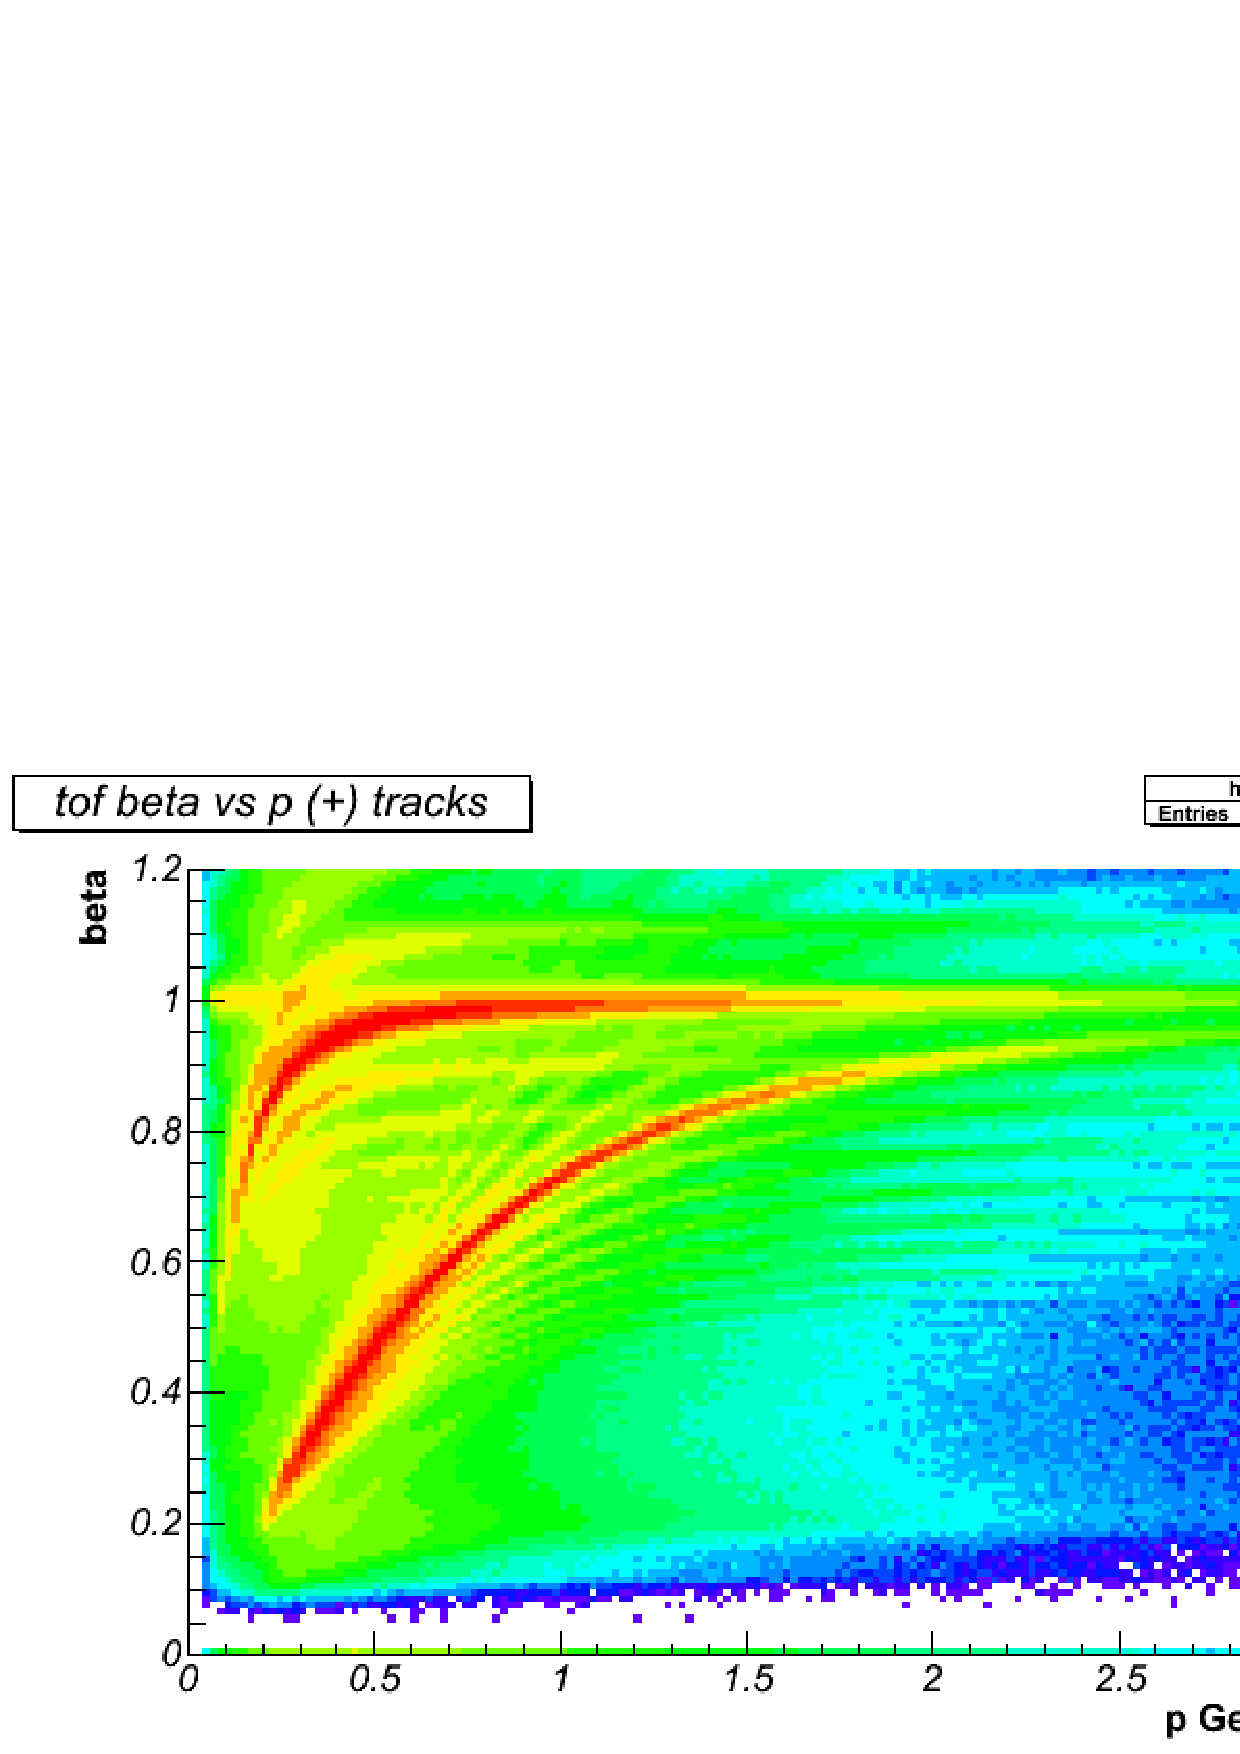
\includegraphics[width=.9\linewidth]{figures/calib/tof/Tof_56855_final_betavpp.pdf}
        \caption{TOF $\beta$ versus momentum for positive tracks}
        \label{plt:tofbetavppos}
    \end{center}\end{subfigure}
\end{center}\end{figure}

\begin{figure}\begin{center}
    \begin{subfigure}{0.5\columnwidth}\begin{center}
        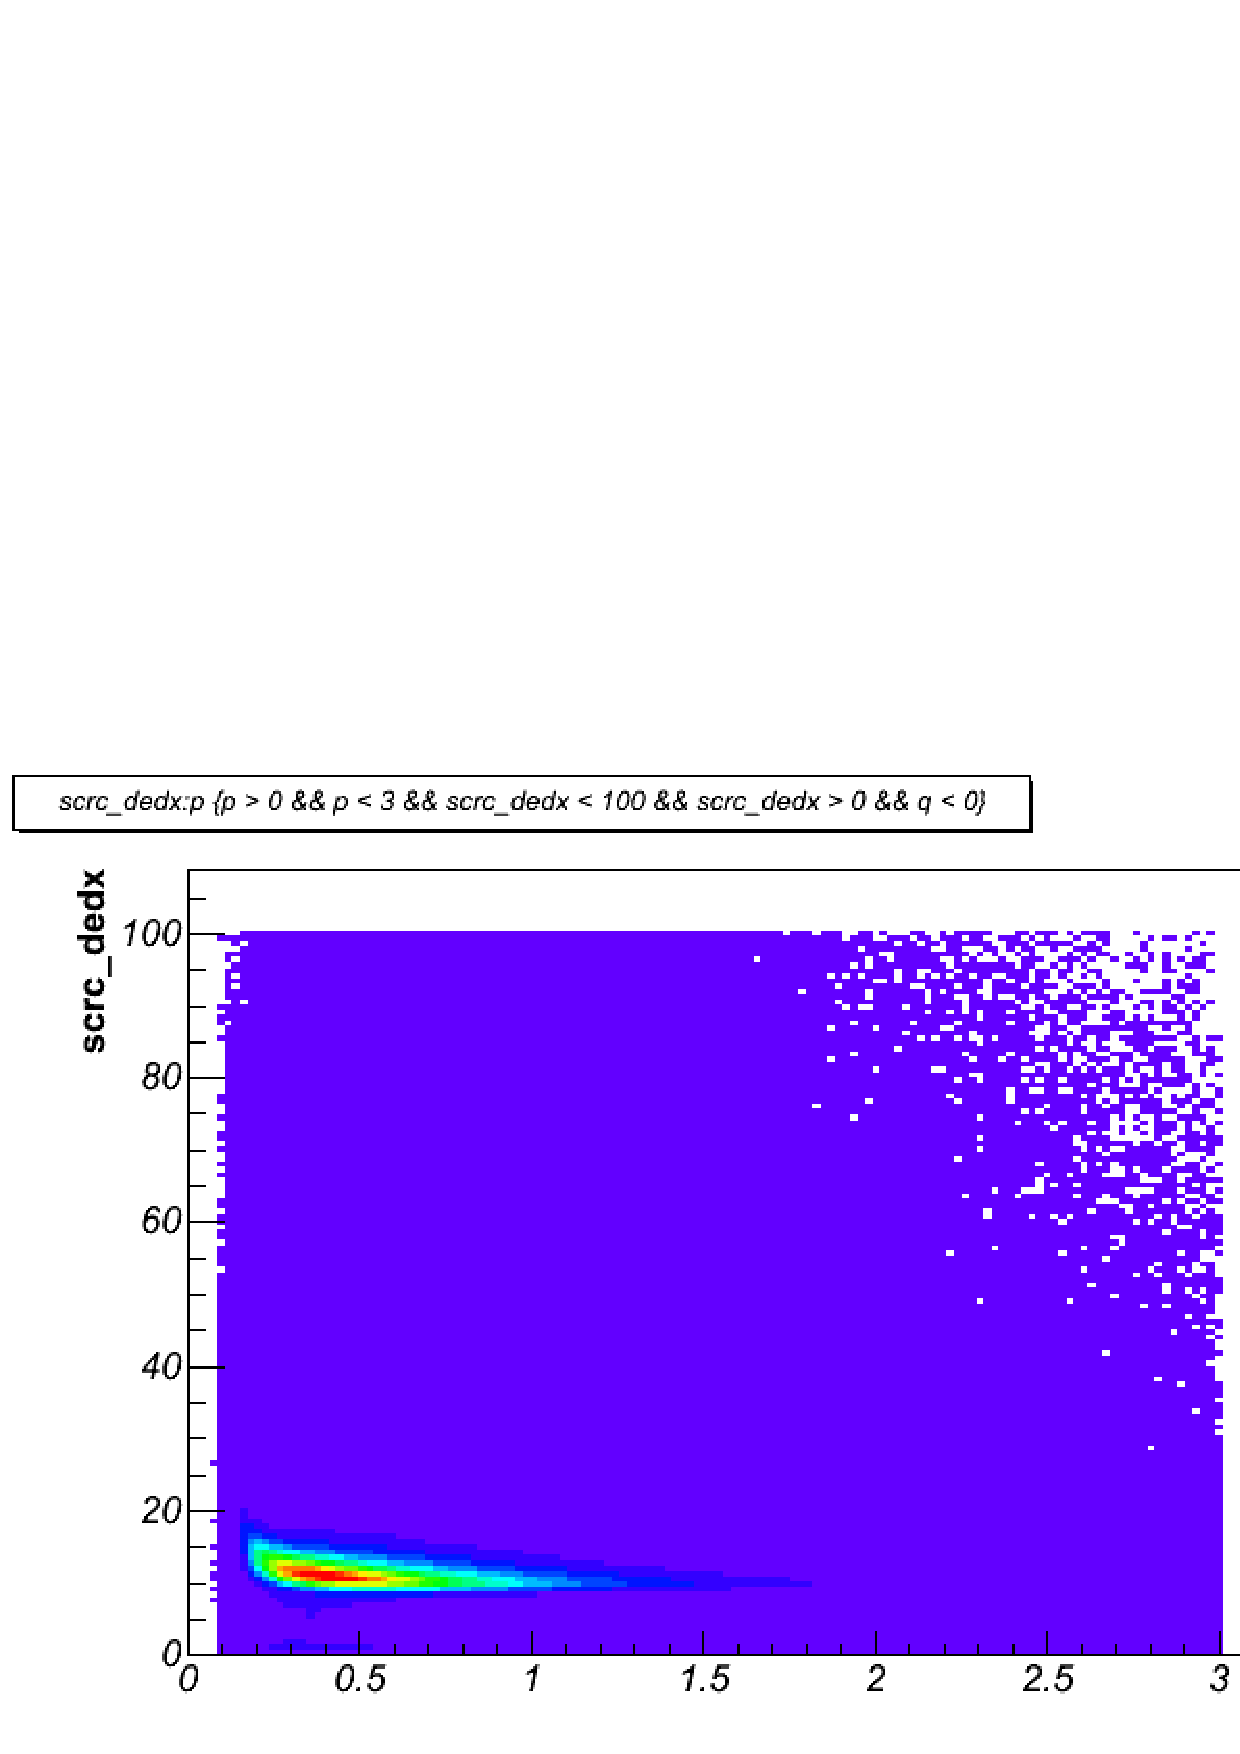
\includegraphics[width=.9\linewidth]{figures/calib/tof/Tof_56855_final_dedxm.pdf}
        \caption{TOF energy deposited versus momentum for negative tracks}
        \label{plt:tofEvpneg}
    \end{center}\end{subfigure}\begin{subfigure}{0.5\columnwidth}\begin{center}
        \includegraphics[width=.9\linewidth]{figures/calib/tof/Tof_56855_final_dedxp.pdf}
        \caption{TOF energy deposited versus momentum for positive tracks}
        \label{plt:tofEvppos}
    \end{center}\end{subfigure}
\end{center}\end{figure}

\begin{figure}\begin{center}
    \begin{subfigure}{0.5\columnwidth}\begin{center}
        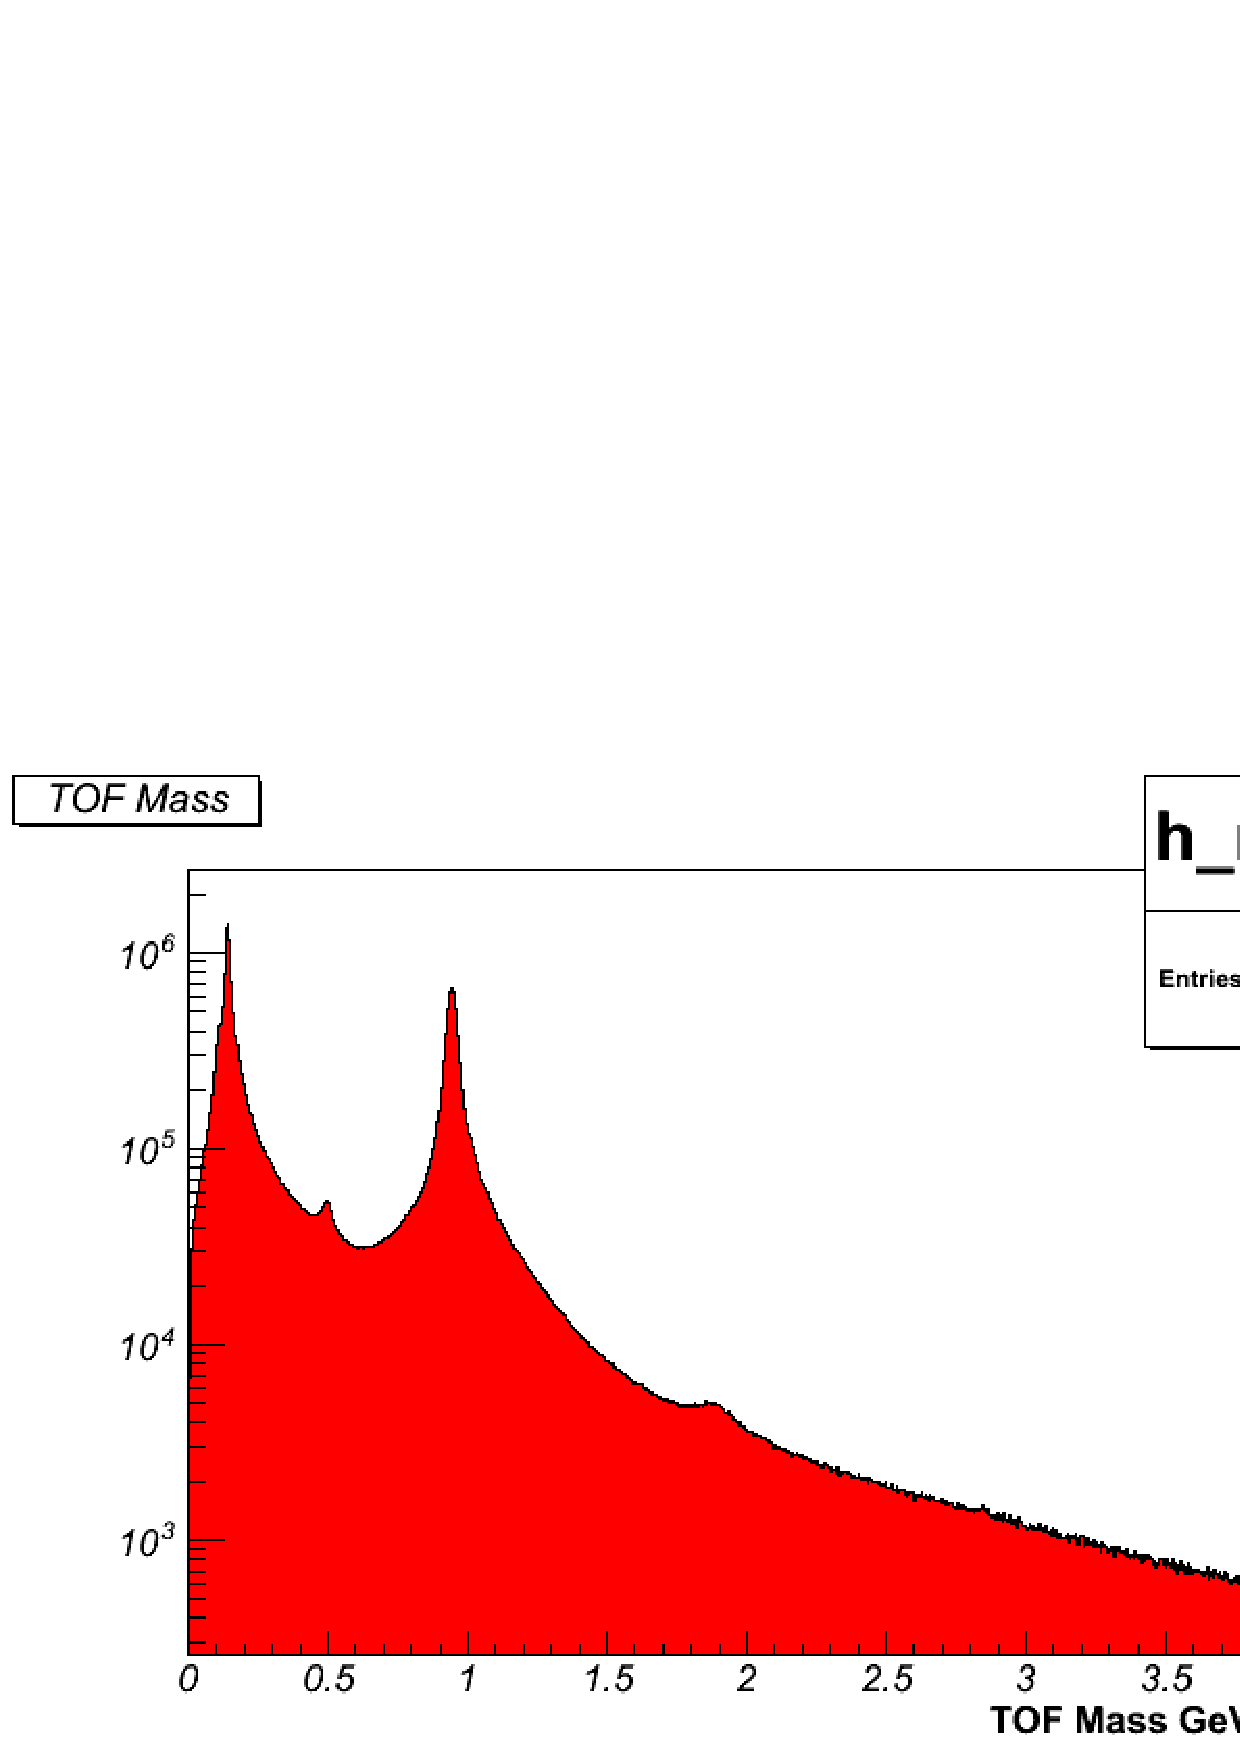
\includegraphics[width=.9\linewidth]{figures/calib/tof/Tof_56855_final_mass.pdf}
        \caption{TOF mass spectrum}
        \label{plt:tofmass}
    \end{center}\end{subfigure}\begin{subfigure}{0.5\columnwidth}\begin{center}
        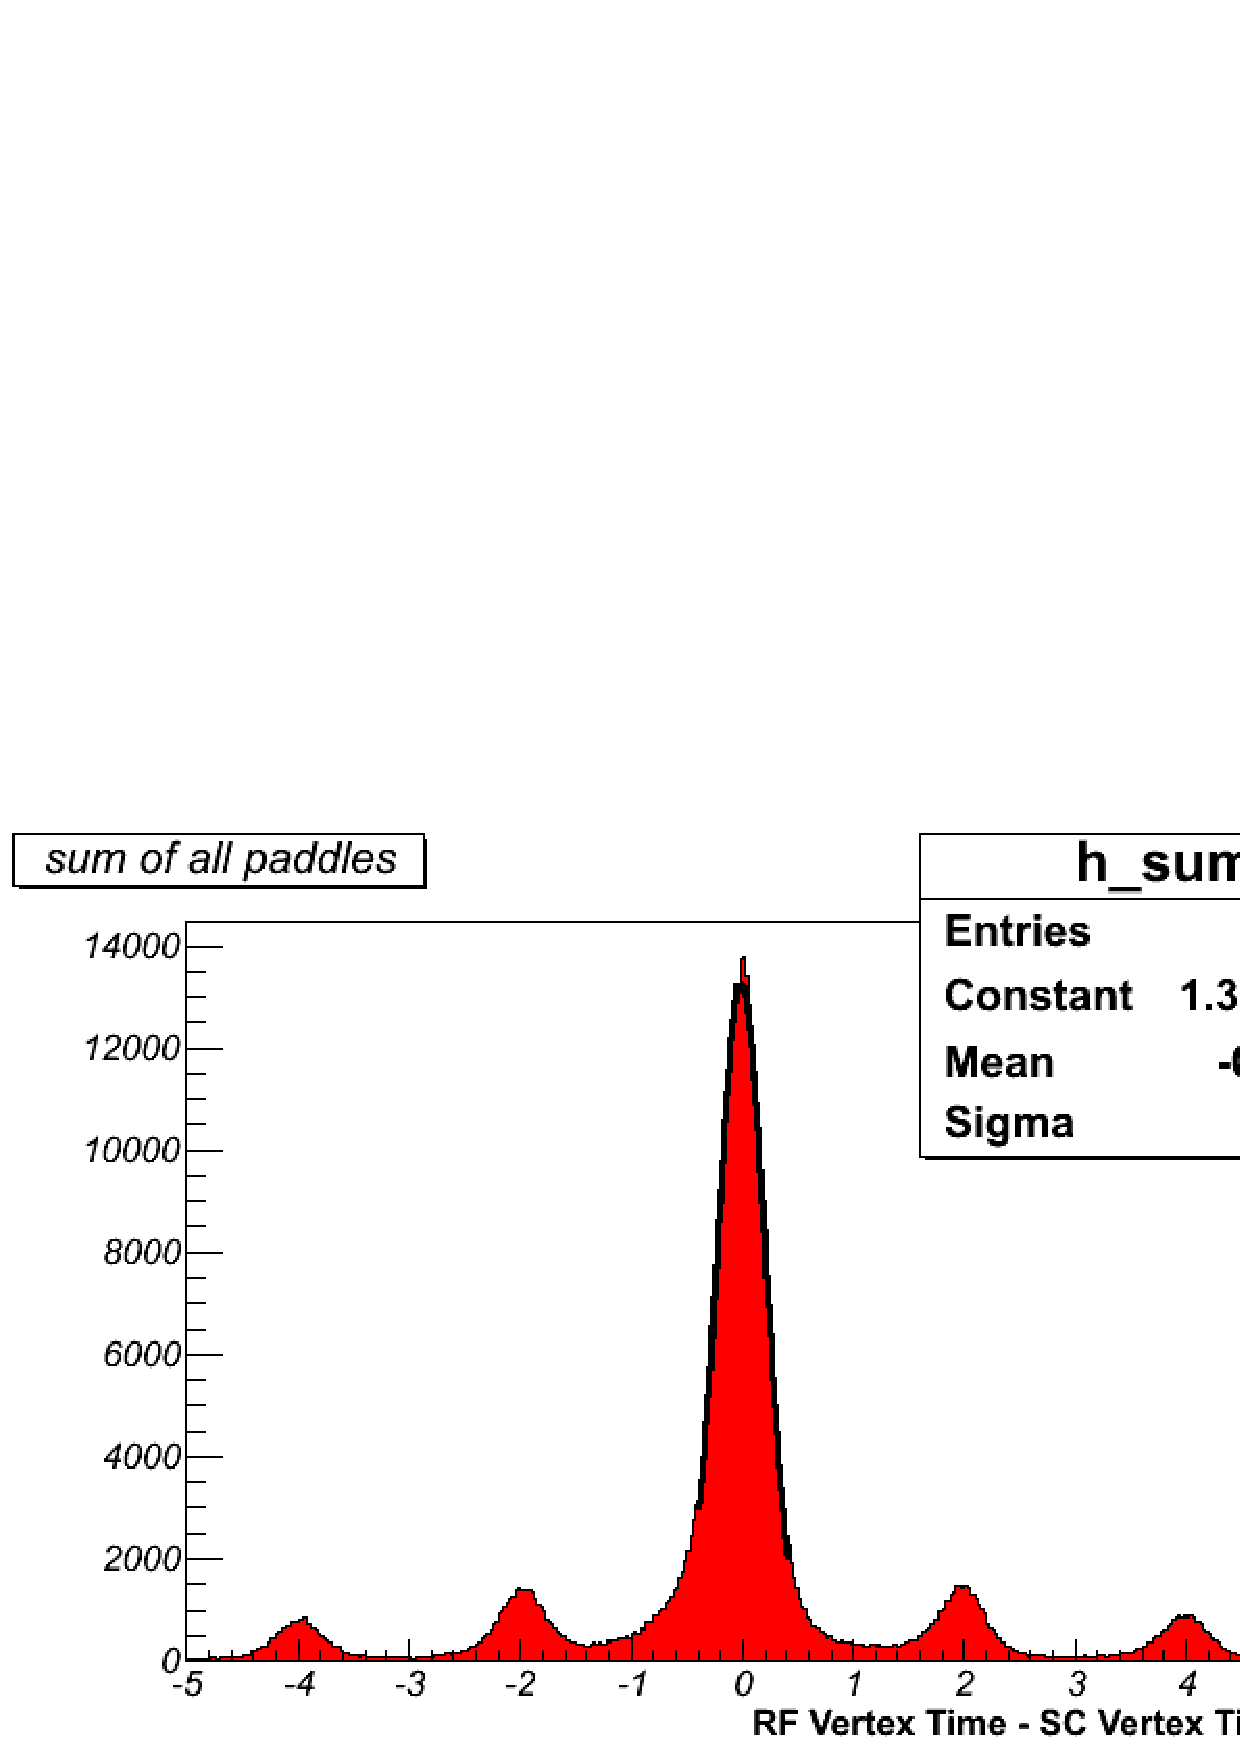
\includegraphics[width=.9\linewidth]{figures/calib/tof/Tof_56855_final_resolution.pdf}
        \caption{TOF resolution integrated over all paddles}
        \label{plt:tofres}
    \end{center}\end{subfigure}
\end{center}\end{figure}

\begin{figure}\begin{center}
    \begin{subfigure}{0.5\columnwidth}\begin{center}
        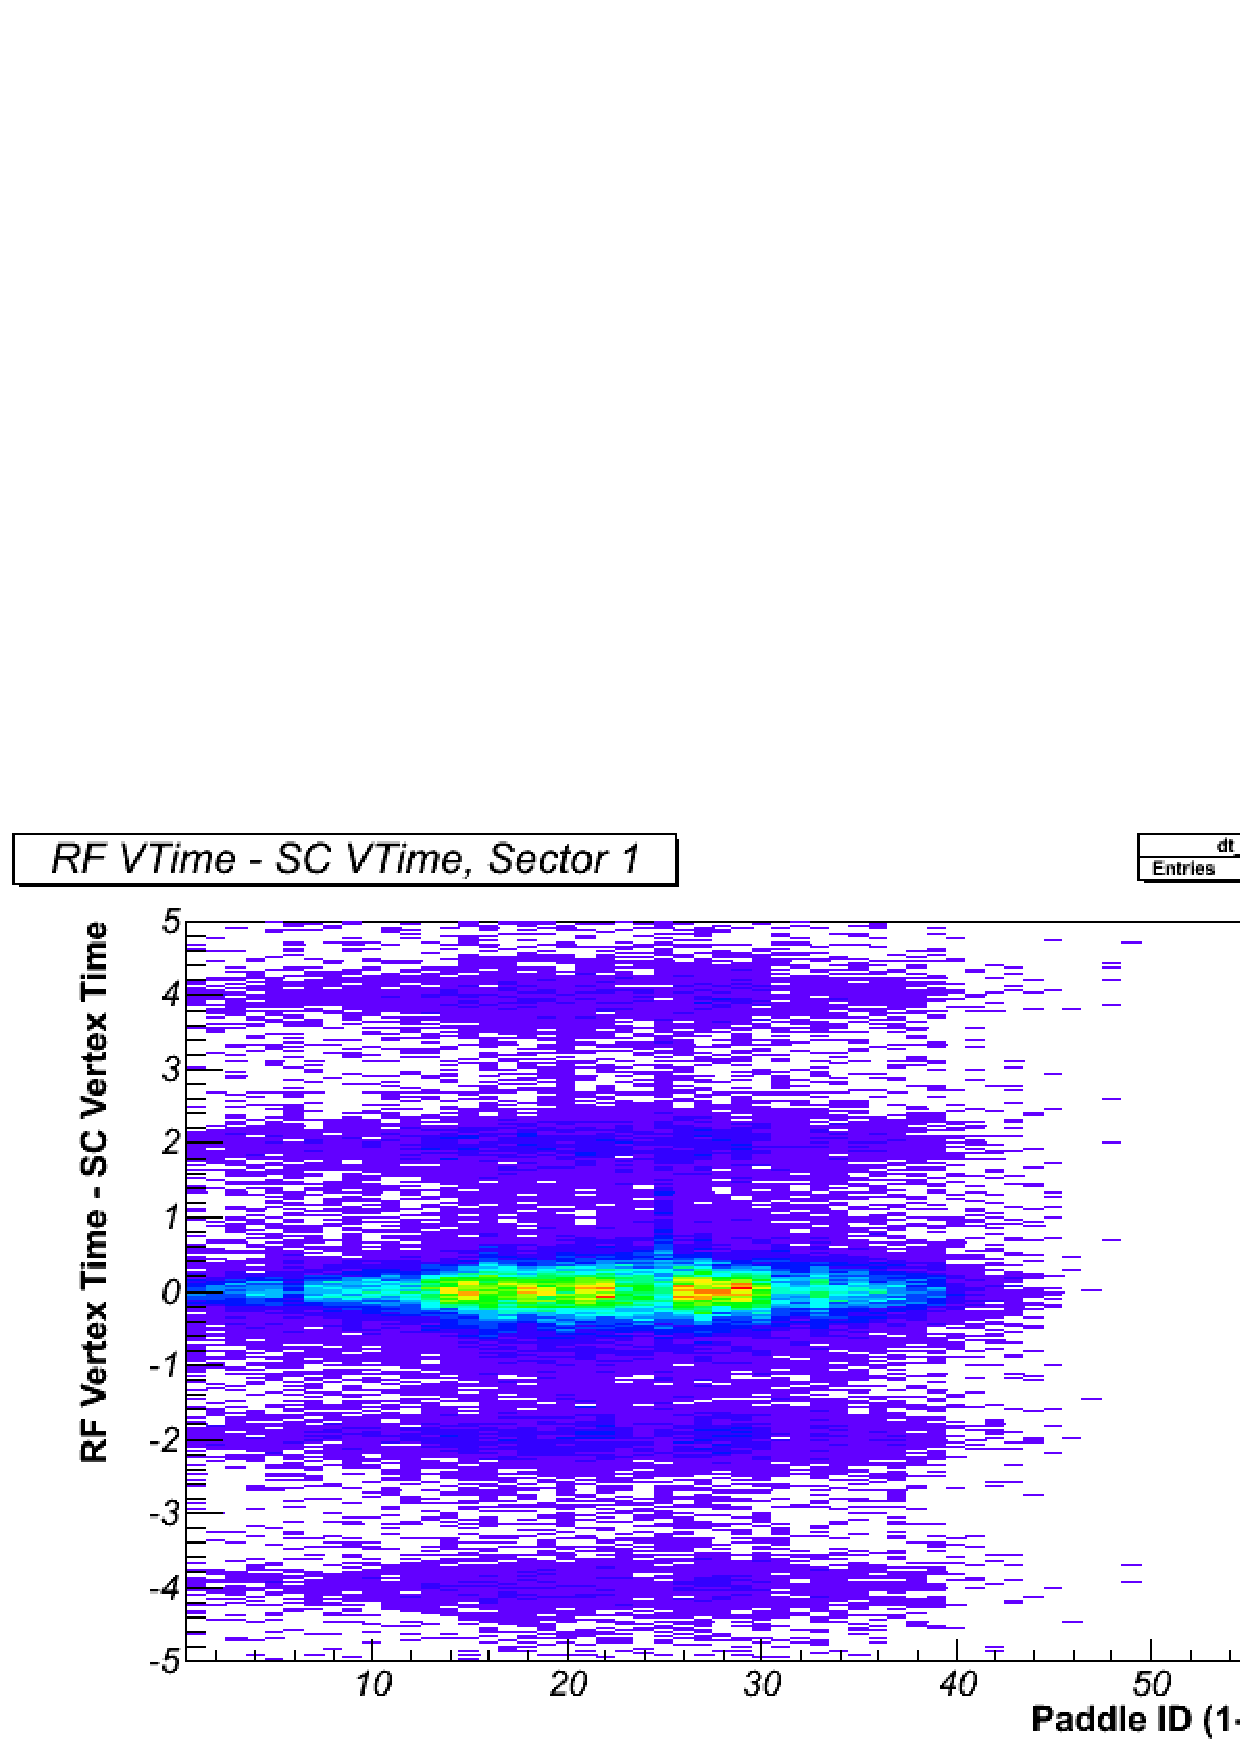
\includegraphics[width=.9\linewidth]{figures/calib/tof/Tof_56855_final_s1p2p.pdf}
        \caption{Representative (sector 1) calibrated timing of the time-of-flight, paddle-by-paddle.}
        \label{plt:tofsec1}
    \end{center}\end{subfigure}\begin{subfigure}{0.5\columnwidth}\begin{center}
        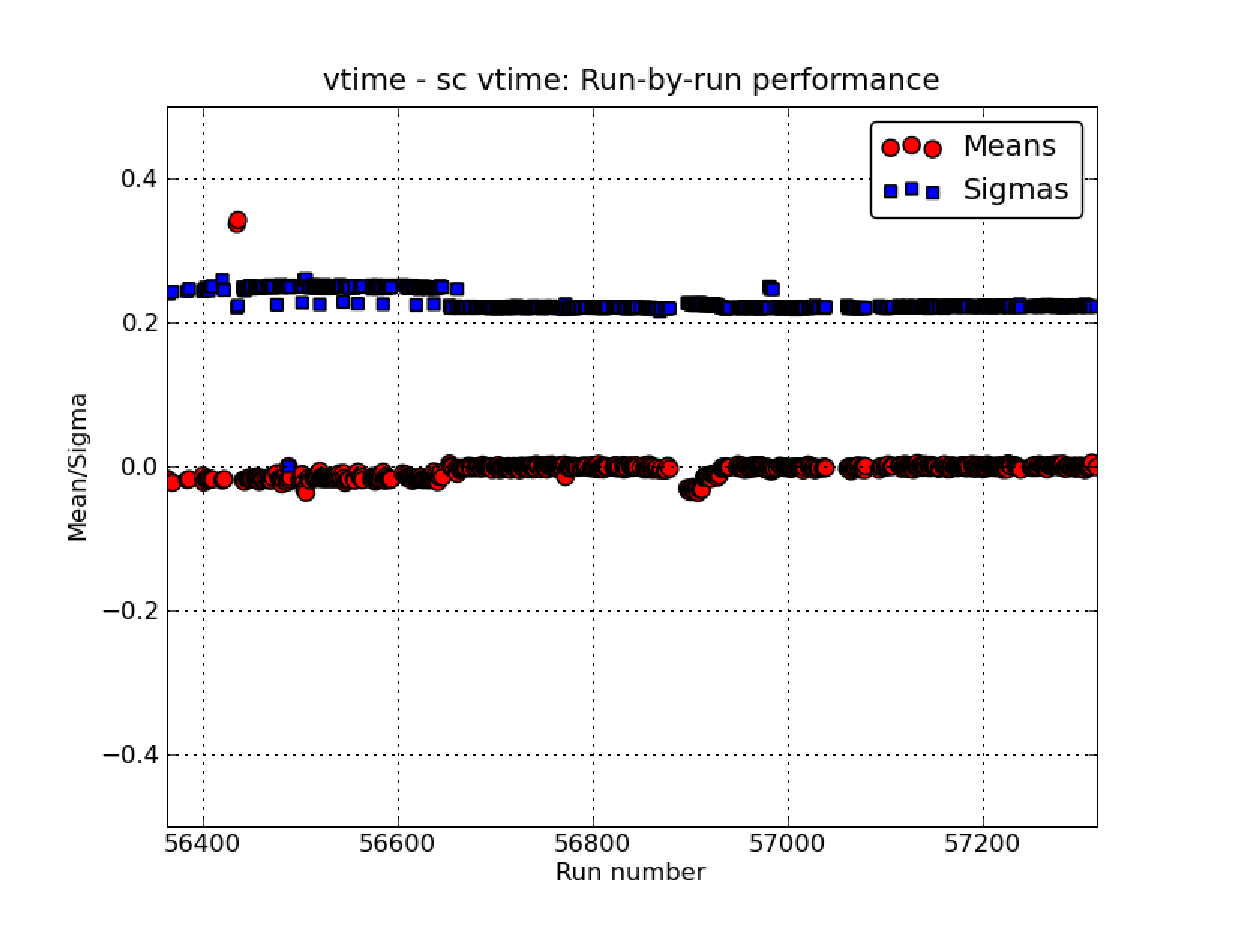
\includegraphics[width=.9\linewidth]{figures/calib/tof/Tof_runscan_p0v7.eps}
        \caption{TOF run-by-run performance}
        \label{plt:tofrunbyrun}
    \end{center}\end{subfigure}
\end{center}\end{figure}

\subsubsection{\label{sec:calib.tof.eff}Time-of-Flight Counter Efficiency and Bad Paddles}

As a standard procedure of the time-of-flight calibrations, the time-of-flight scintillators were initially studied during the calibration period, in which a list~\footnote{Can be obtained using the CLAS calibration database} of scintillators had a faulty ADC or TDC as shown in Table~\ref{tab:craigtof}. Another study, as shown below, was conducted to determine the efficiency of each paddle and to reevaluate the status of their ADC and TDC. Due to the more stringent requirements of paddle efficiency in the study below, more paddles were considered to be faulty than in the initial study. Table~\ref{tab:diff} shows the additional paddles which were considered to be inefficient.

\begin{table}
\begin{minipage}{\textwidth}
\begin{center}
\begin{singlespacing}

\caption{\label{tab:craigtof}List of faulty paddles as compiled during calibration}
    
\begin{tabular}{llp{.43\textwidth}}

\hline \hline

Sector & SCID & Notes \\

\hline

1 & 6 & No ADCR and TDCR \\
2 & 8 & No ADCL and TDCL \\
2 & 34 & No ADCL and TDCL \\
3 & 11 & No ADCR and TDCR \\
3 & 57 & No ADCL, ADCR, TDCL, and TDCR \\
4 & 48 & No ADCL and TDCL \\
5 & 57 & No ADCL, ADCR, TDCL, and TDCR \\
6 & 5 & No ADCR and TDCR \\

\hline \hline

\end{tabular}

\end{singlespacing}
\end{center}
\end{minipage}
\end{table}
 % label: tab:craigtof

\begin{figure}\begin{center}
    \includegraphics[trim=0 40 10 40,clip,width=.40\linewidth]{figures/calib/tof/tofko/occp.eps}
    \caption{Relative occupancy of all scintillators}
    \label{plt:occp}
\end{center}\end{figure}

To determine efficiency of each scintillator paddle, the number of hits~\footnote{The data used were obtained from the \texttt{clas\underline{\hspace{5pt}}0$[$run\#$]$.A01} files located in \texttt{$/$mss$/$clas$/$g12$/$data$/$}} registered by every paddle was recorded~\footnote{This was done by using \texttt{bosdump -GSC} and parsing its output}. The relative occupancy of paddle $i$ in sector $j$ is defined the following way: list the number of hits recorded by all paddle $i$'s in sectors $\neq j$ and remove the ones with the most and least hits from the list. Take the average number of hits of the remaining three paddles. The relative occupancy is defined as
\[
100 \times \frac{ \mathrm{Number of hits in paddle } i \mathrm{ of sector } j}{\mathrm{Average of remaining three paddles}} \hspace{2pt}\%
\]

Fig.~\ref{plt:occp} shows the relative occupancy of all scintillators plotted on a single histogram. A paddle is defined as inefficient if it is greater than two standard deviations below the mean relative occupancy of all scintillators. Table.~\ref{tab:occp} shows the paddles which are below two (left) or three (right) standard deviations below the mean relative occupancy.

\begin{table}
\begin{minipage}{\textwidth}
\begin{center}
\begin{singlespacing}

\caption{\label{tab:occp}Paddles below two and three standard deviations from the mean relative occupancy}

\begin{tabular}{lcc}

\hline \hline

 &  $2 \sigma = 92.49\%$ &  $3 \sigma = 89.05\%$ \\
 
\hline

Sector 1 & 35 (91.20\%) & 40 (87.87\%), 41 (82.63\%), 56 (83.37\%) \\
Sector 2 & 2 (92.38\%), 35 (90.11\%), 50 (91.99\%) &  41 (87.31\%), 56 (87.98\%)\\
Sector 3 & 35 (90.59\%) & 40 (88.98\%), 41 (83.29\%)\\
Sector 4 &  & 41 (83.61\%) \\

\hline \hline

\end{tabular}

\end{singlespacing}
\end{center}
\end{minipage}
\end{table}
 % label: tab:occp

\subsubsection{\label{sec:calib.tof.adctdc}ADC and TDC Values}

\begin{figure}\begin{center}
    \includegraphics[width=0.70\linewidth]{figures/calib/tof/tofko/adctdcval.eps}
    \caption{\label{plt:adctdcval}Top: ADC values of all scintillators. Left ADC (ADCL) values are on the left and right ADC values are on the right (ADCR). Shaded in red are events recorded with an ADC value of zero or maximum. Bottom: Same as Top but for TDC values}
\end{center}\end{figure}

The occupancy alone is not enough to determine which scintillators are bad. The ADC and TDC values for all scintillators were also recorded and studied. Fig.~\ref{plt:adctdcval} shows the ADC and TDC values for all scintillators. Some of the events registered had an ADC or TDC value of zero or a maximum ADC value (shaded in red). The percentage of events a scintillator recorded either a TDC or ADC value of zero or maximum ADC value was studied as shown in Figs.~\ref{plt:adc0vSCID}, \ref{plt:adcMvSCID} and \ref{plt:tdc0vSCID}. Figures~\ref{plt:adc0vSCID}, \ref{plt:tdc0vSCID} and \ref{plt:proj} assisted in determining bad paddles. It (is to be) was decided that a paddle cannot have more than $50\%$ of its ADC (left or right) values be equal to zero or more than $45\%$ of its TDC (left or right) values equal to zero. Table~\ref{tab:adctdc0} shows which paddles fall in these categories. Table~\ref{tab:tofko} shows which scintillators should be knocked out due to low occupancy or too many null ADC or TDC values. Due to the small number of events in which a maximum ADC value is obtained, it is not recommended in knocking paddles out based on this measure. However, Table~\ref{tab:adcM} shows the paddles which attain a maximum ADC value on more than $2.5\%$ of its registered events.

\begin{table}
\begin{minipage}{\textwidth}
\begin{center}
\begin{singlespacing}

\caption{\label{tab:adctdc0}Paddles which registered an ADC or TDC value of zero greater than 50\% and 45\%, respectively, of its entries}

\begin{tabular}{lp{.43\textwidth}p{.43\textwidth}}

\hline \hline

 &  \% Events with ADCL or ADCR = 0 \( > \) 50\% &  \% Event with TDCL or TDCR = 0 \( > \) 45\% \\
 
\hline

Sector 1 & 6 (100\% ADCR) & 6 (100\% TDCR), 46 (97.89\% TDCL), 50 (98.11\% TDCL) \\
Sector 2 & 8 (100\% ADCL), 34 (100\% ADCL), 44 (50.22\% ADCL), 54 (52.00\% ADCR) &  8 (100\% TDCL), 34 (100\% TDCL), 44 (47.51\% TDCL), 54 (47.10\% TDCR)\\
Sector 3 & 11 (100\% ADCR), 56 (74.75\% ADCR) & 11 (100\% TDCR), 56 (62.79\% TDCR)\\
Sector 4 & 48 (100\% ADCL) & 48 (100\% TDCL) \\
Sector 5 & 48 (77.98\% ADCL) & 48 (76.10\% TDCL)\\
Sector 6 & 5 (100\% ADCR), 56 (59.30\% ADCR) & 1 (98.78\% TDCL), 5 (100\% TDCR), 33 (97.78\% TDCL) \\

\hline \hline

\end{tabular}

\end{singlespacing}
\end{center}
\end{minipage}
\end{table}
 % label: tab:adctdc0

\begin{table}
\begin{minipage}{\textwidth}
\begin{center}
\begin{singlespacing}

\caption{\label{tab:tofko}Union of \ref{tab:occp,tab:adctdc0} (Recommended list of paddles to knockout)}

\begin{tabular}{lc}

\hline \hline

Sector 1: & 6, 35, 40, 41, 50, 56\\
Sector 2: & 2, 8, 34, 35, 41, 44, 50, 54, 56\\
Sector 3: & 11, 35, 40, 41, 56\\
Sector 4: & 41, 48 \\
Sector 5: & 48\\
Sector 6: & 1, 5, 33, 56 \\

\hline \hline

\end{tabular}

\end{singlespacing}
\end{center}
\end{minipage}
\end{table}

 % label: tab:tofko

\begin{table}
\begin{minipage}{\textwidth}
\begin{center}
\begin{singlespacing}

\caption{\label{tab:diff}Paddles in \ref{tab:tofko} not included in \ref{tab:craigtof}}

\begin{tabular}{lc}

\hline \hline

Sector 1: & 35, 40, 41, 50, 56 \\
Sector 2: & 2, 35, 41, 44, 50, 54, 56 \\
Sector 3: & 35, 40, 41, 56 \\
Sector 4: & 41 \\
Sector 5: & 48 \\
Sector 6: & 1, 33, 56 \\

\hline \hline

\end{tabular}

\end{singlespacing}
\end{center}
\end{minipage}
\end{table}
 % label: tab:diff

\begin{table}
\begin{minipage}{\textwidth}
\begin{center}
\begin{singlespacing}

\caption{\label{tab:adcM}Paddles with percentage of hits registering a maximum ADC value \( > \) 2.5\% of its events}

\begin{tabular}{lc}

\hline \hline

Sector 1: & 20 (2.93\% ADCL) \\
Sector 3: & 20 (4.26\% ADCL) \\

\hline \hline

\end{tabular}

\end{singlespacing}
\end{center}
\end{minipage}
\end{table}

 % label: tab:adcM

\begin{figure}\begin{center}
    \includegraphics[width=0.75\textwidth]{figures/calib/tof/tofko/adc.eps}
    \caption{\label{plt:adc0vSCID}Percentage of hits registering an ADC value of 0 for all scintillators. Left ADC (ADCL) are on the left and right ADC (ADCR) values are on the right}
\end{center}\end{figure}

\begin{figure}\begin{center}
    \includegraphics[width=0.75\textwidth]{figures/calib/tof/tofko/tdc.eps}
    \caption{\label{plt:tdc0vSCID}Percentage of hits registering an TDC value of 0 for all scintillators. Left TDC (TDCL) are on the left and right TDC (TDCR) values are on the right}
\end{center}\end{figure}

\begin{figure}\begin{center}
    \includegraphics[width=0.75\textwidth]{figures/calib/tof/tofko/adcMax.eps}
    \caption{\label{plt:adcMvSCID}Percentage of hits registering a maximum ADC value for all scintillators. Left ADC (ADCL) are on the left and right ADC (ADCR) values are on the right}
\end{center}\end{figure}

\begin{figure}\begin{center}
    \includegraphics[width=0.8\textwidth]{figures/calib/tof/tofko/adctdc0perc.eps}
    \caption{\label{plt:proj}Top: Y axis projections of Fig.~\ref{plt:adc0vSCID}. Bottom: Y axis projections of Fig.~\ref{plt:tdc0vSCID}}
\end{center}\end{figure}

\begin{v2}
\subsubsection{\label{sec:calib.tof.resolution}Time-of-Flight Paddle Resolution}
So far, the selection of bad paddles is based only the raw data, which is only good for the initial selection. We further investigate the timing resolution of each paddle by run in order to determine stability of their resolutions throughout the experiment. The following data analyzed were from events containing $p \pi^{+} \pi^{-}$ in the final state. For the $\pi^{+}$ and $\pi^{-}$, the difference between the measured time-of-flight and the expected time-of-flight for a given run was plotted and fitted to a Gaussian. This was done for every paddle and every run. We define the resolution of that paddle to be the standard deviation of the fit. 
%Figure~\ref{plot:example.tofresVrun} shows an example of this. The TOF resolution for every paddle as a function of run number is stored in the g12 wiki page. 
A few paddles that had not been previously knocked out had drifts on either the resolution or the mean $\Delta$ TOF and were not properly calibrated. Table~\ref{tab:tofko.additional} shows which paddles should ideally be knocked out due to this. However, the track dependent efficiency correction was derived without these paddles being knocked out. Consequently, the these paddles should not be knocked out if using the track dependent efficiency correction. If one would like to use these additional time-of-flight knockouts, then one would need to re-derive the track dependent efficiency corrections. Figure~\ref{plot:example.goodpaddle} shows an example of a good paddle's resolution and mean $\Delta$ TOF while figure~\ref{plot:example.badpaddle} shows and example of a bad paddle. The TOF resolution for every paddle by run is stored in the g12 wiki.


\begin{figure}\begin{center}
      \includegraphics[width=0.95\columnwidth]{figures/calib/tof/goodexample.pdf}
   \caption{\label{plot:example.goodpaddle}TOF resolution as a function of run number for a good paddle}
\end{center}\end{figure}

\begin{figure}\begin{center}
      \includegraphics[width=0.95\columnwidth]{figures/calib/tof/badexample.pdf}
   \caption{\label{plot:example.badpaddle}TOF resolution as a function of run number for a bad paddle}
\end{center}\end{figure}
\end{v2}

\FloatBarrier

\subsection{\label{sec:calib.ec}Electrocalorimeter Calibration and Resolution}

\subsubsection{\label{sec:calib.ec.eff}Electrocalorimeter Efficiency and Bad Paddles}

\FloatBarrier

\subsection{\label{sec:calib.pol}Beam Polarization}
The electron beam produced with a polarized laser incident on gallium arsenide allows for longitudinal polarization of the electrons~\cite{polarizedelectrons} and in turn, due to the bremsstrahlung process, circular polarization of the photon beam.  The accurate measurement of the polarization transferred from the photon beam to the produced hyperons ($C_x$ and $C_z$) requires knowledge of the beam polarization.  Such knowledge is ascertained by knowing the magnitude of incident electron-beam polarization, and the helicity orientation of the electron beam bunch responsible for the event (in the lab-frame). The Maximon-Olsen formula relating incident electron beam polarization, with the photon polarization is given by~\cite{MaximonOlsen},
\begin{equation}
P_\odot(E_\gamma) = \frac{x(4-x)}{4 - 4x + 3x^2}P_{elec}
\end{equation}
where $x = E_\gamma /E_{elec}$ is the ratio of photon energy, $E_\gamma$, to beam energy, $E_{elec}$. The g12 experiment ran with a constant electron energy of $E_{elec} = 5.715$ GeV.  (The actual electron beam energy was corrected on a run-by-run basis, see later section) The polarization of the electron beam was measured regularly using the a M{\o}ller polarimeter.  The polarimeter measures electron polarization by making use of the helicity dependent nature of M{\o}ller scattering~\cite{Mecking,Carman}. The M{\o}ller measurements, summarized in Fig.~\ref{moltable}, were performed regularly (every few days) during g12.  The run-integrated and flux -weighted value of the polarization of a particular range of photon energies can be easily obtained by using the maximum-Olsen formula.

\begin{figure}[h]
\begin{center}
 \includegraphics[width=0.9\textwidth]{figures/calib/pol/moltable.eps}
  \caption{The degree of longitudinal electron polarization ($P_e)$ for each M{\o}ller run. }
  \label{moltable}
  \end{center}
\end{figure}



An important experimental aspect of g12 is that the electron-beam helicity was flipped at a rate around 30 Hz. While the helicity information was recorded and stored in the HEVT bank for each event, the convention for bit encoding has been known to change from real-time to delayed-time recording. Further considerations, such as the half-wave plate orientation also had to be accounted for.

The only sure way to pin down the absolute beam helicity orientation for our data was to analyze a well known helicity-dependent reaction. Well-established results in Ref.~\cite{Io} in the beam-helicity asymmetry, $I^\odot(\phi^{hel}_\pi)$, for the reaction, $\gamma p \to p \pi^+ \pi^-$, were reproduced.  The mentioned reaction was shown to have a specific helicity-frame defined $\phi^{hel}_{\pi^+}$-dependent structure.  If the helicity convention was reversed then we would observe $I^\odot(\phi^{hel}_{\pi^+}) \to -I^\odot(\phi^{hel}_{\pi^+})$.

The sub-analysis we performed required exclusive $p \pi^+ \pi^-$ events in the final state. To ensure exclusivity we required zero missing energy and momentum within detector resolution. The helicity frame (shown in Fig.~\ref{ioplane}) was defined to be the rest frame of the hypothetical parent meson of the two pion system, with  $\hat{z}$ aligned along its center-of-mass defined momentum. $\phi^{hel}_{\pi^+}$ is the angle between the proton-production plane, and the plane containing both pions. The beam helicity asymmetry is given by,
\begin{equation}
I_\odot = \frac{N^+ - N^-}{N^+ + N^-},
\end{equation}
where $N^\pm$ indicates the number of events with positive (negative) photon helicity.  Figs.~\ref{myIo}-\ref{Io} show the $I_{\odot}(\phi^{hel}_{\pi^+})$ for g12 and in the analysis of \cite{Io}.
The lab-frame electron helicity readout was taken from the HEVT bank (HEVT$\to$hevt[0].TGRPRS). The results of our $I_{\odot}(\phi^{hel}_{\pi^+})$ analysis and the previously published results showed a positive (negative) HEVT readout indicates positive (negative) photon helicity. The reproduction of beam-helicity asymmetry for double charged pion production also served as a way to test the accuracy of the calculated photon polarization magnitude: both results' wave amplitudes were in good agreement.

\begin{figure}[h]
\begin{center}
 \includegraphics[width=0.9\textwidth]{figures/calib/pol/ioplane.eps}
  \caption{An illustration of the angle definitions used in the $\gamma p \to \pi^+ \pi^- p$ sub-analysis. $\theta_{cm}$ is defined in the center-of-mass frame. $\theta$ and $\phi$ are defined in the rest frame of the $\pi^+$ $\pi^-$ system as the polar and azimuthal angles. The $z$ direction is along the total momentum of the $\pi^+ \pi^-$ system.}
  \label{ioplane}
  \end{center}
\end{figure}


\begin{figure}[h]
\begin{center}
 \includegraphics[width=0.9\textwidth]{figures/calib/pol/myIo.eps}
  \caption{$I_{\odot}(\phi^{hel}_{\pi^+})$ for g12 data within the energy range of $W = 1.9-2.3$ GeV.}
  \label{myIo}
  \end{center}
\end{figure}


\begin{figure}[h]
\begin{center}
 \includegraphics[width=0.9\textwidth]{figures/calib/pol/Io.eps}
  \caption{$I_{\odot}(\phi^{hel}_{\pi^+})$ as measured in the previous analysis.}{ $I_{\odot}(\phi^{hel}_{\pi^+})$ as measured in the analysis~\cite{Io}. The results of are shown in bins of $W$ from $1.9$ to 2.3 GeV.}
  \label{Io}
  \end{center}
\end{figure}




To conclude, the g12 beam polarization was measured with standard methods, and the validity of the photon helicity definition in the HEVT bank was double checked against existing experimental results and confirmed to be correct. All g12 measurements that utilizes the beam polarization refer to what has been summarized here.



